%% =====================================================================
%%  IEEE SPMB 2026 — SUBMISSION-READY v4 (single-author)
%%  ESF: A Canonical Representation and Recoverability Framework
%%       for Deploying Pretrained EEG Classifiers in Heterogeneous
%%       Clinics
%%
%%  Sole author: Hitesh Dammu (Independent Researcher, Hyderabad, India)
%%
%%  Numerical claims reproduce from
%%    /Users/h/Desktop/SPMB/data/sweep_tuab_final.csv  (46 rows, 5 axes)
%%    /Users/h/Desktop/SPMB/data/per_recording_failure_profile.csv (n=276)
%%    /Users/h/Desktop/SPMB/theory/validation_summary.json
%% =====================================================================

\documentclass[conference]{IEEEtran}

\IEEEoverridecommandlockouts
\ifCLASSINFOpdf
\else
\fi
\usepackage{amsmath,graphicx,soul,subcaption,balance}
\usepackage[numbers,sort&compress]{natbib}
\renewcommand\bibsection{\section*{\normalsize References}}
\usepackage{float}
\usepackage{times}

\usepackage{multirow}
\usepackage{color}
\usepackage{soul,mathrsfs}
\usepackage[utf8]{inputenc}
\usepackage[T1]{fontenc}
\usepackage{array}
\usepackage[hyphens, spaces, obeyspaces]{url}
\def\UrlFont{\em}

\usepackage{booktabs}
\usepackage[table]{xcolor}
\usepackage{amssymb,amsfonts}
\usepackage{amsthm}
\usepackage{tikz}
\usetikzlibrary{positioning,arrows.meta,shapes.geometric,calc}

\newcolumntype{L}[1]{>{\raggedright\let\newline\\\arraybackslash\hspace{0pt}}m{#1}}
\newcolumntype{C}[1]{>{\centering\let\newline\\\arraybackslash\hspace{0pt}}m{#1}}
\newcolumntype{R}[1]{>{\raggedleft\let\newline\\\arraybackslash\hspace{0pt}}m{#1}}

\usepackage{caption}
\captionsetup[figure]{font=small,name=Fig.}
\captionsetup[table]{font=small,name=TABLE}
\renewcommand{\thetable}{\arabic{table}}

\captionsetup{justification=justified,singlelinecheck=true}
\captionsetup{belowskip=0pt}

\usepackage{colortbl}
\definecolor{light-gray}{gray}{0.83}
\newcommand{\GREY}{\cellcolor{light-gray}\bf}




\hyphenation{op-tical net-works semi-conduc-tor canon-ical-iza-tion
acqui-si-tion recover-ability}

\graphicspath{{../figures/}{./figures/}{./}}

\usepackage{fancyhdr,lastpage}
\fancyhf{}
\renewcommand{\headrulewidth}{0pt}
\fancypagestyle{firststyle}
{
   \fancyhf{}
   \fancyfoot[L]{\scriptsize Preprint v2, Sept.\ 2026. v1 (30 June 2026) was submitted to IEEE SPMB 2026 and withdrawn by the author; see Version note.}
   \fancyfoot[R]{\scriptsize Code: doi:10.5281/zenodo.22771925}
   \fancyfoot[C]{}
}
\thispagestyle{firststyle}
\pagestyle{fancy}
\fancyhf{}
% Running header intentionally empty — the IEEE-template default running
% title isn't required by the SPMB CFP and adds noise to a 6-page paper.
% The IEEE copyright + conference plate stay in the footer per template.
\fancyfoot[L]{\scriptsize Preprint v2, Sept.\ 2026. v1 (30 June 2026) was submitted to IEEE SPMB 2026 and withdrawn by the author; see Version note.}
\fancyfoot[R]{\scriptsize Code: doi:10.5281/zenodo.22771925}
\fancyfoot[C]{}

% theorem environments
\newtheorem{definition}{Definition}
\newtheorem{proposition}{Proposition}
\newtheorem{theorem}{Theorem}

%%%%%%%%%%%%%%%%%%%%%%%%%%%%%%%%%%%%%%%%%%%%%%%%%%%%%%%%%%%%%%%%%%%%%%%%%%%
\title{ESF: Harmonizing Heterogeneous EEG Acquisition\\for Pretrained Classifiers}
\author{\IEEEauthorblockN{Hitesh Dammu}
\IEEEauthorblockA{Independent Researcher, Hyderabad, India \\
hdammu@asu.edu}}

\newcommand{\PaperTitleSummary}{Dammu: ESF, harmonizing heterogeneous EEG acquisition for pretrained classifiers}


\newcommand{\PINSKERNUMBERS}{The class-conditional bound of Theorem~\ref{thm:tv} holds on all $40$ measured arms for every model, and the label-free (marginal) version has no constant below $1$ on any of them (Appendix~A.4): the marginal shift a deployed system can see does not bound its loss.}
\newcommand{\PINSKERLABRAM}{, $40/40$ for LaBraM}
\newcommand{\BANDWIDTHABS}{ So does LaBraM's.}
\newcommand{\LABRAMPERM}{, $0.48 \pm 0.10$ (LaBraM; linear $0.51$)}
\newcommand{\LABRAMABS}{ LaBraM sits between: $128$\,Hz is not recovered either ($0.89 \to 0.82$), while $512$\,Hz and mains are.}
\newcommand{\LABRAMDISC}{ LaBraM fails at $128$\,Hz too, and its $64$\,Hz low-pass cell reproduces that failure exactly.}
\newcommand{\LABRAMAONE}{ LaBraM is a third case: $200$ and $512$\,Hz are recovered (naive $0.845$ and $0.608$ to canonicalized $0.898$ and $0.895$, $p = 3\times10^{-4}$ and $2\times10^{-10}$), but $128$\,Hz is not, and resampling does nothing for it (naive $0.813$, canonicalized $0.815$, balanced accuracy $0.50$).}
\newcommand{\LABRAMATWO}{ LaBraM's naive arm is already tolerant of gain (losses $\le 0.02$, none significant).}
\newcommand{\LABRAMATHREE}{ LaBraM's naive arm falls to $0.863/0.801/0.786/0.681$ and, unlike the other two, pushes \emph{abnormal} recordings toward normal (\S\ref{sec:failure}).}
\newcommand{\LABRAMAFOUR}{ LaBraM loses most, $0.044$ on \texttt{legacy16} with balanced accuracy $0.53$.}
\newcommand{\LABRAMAFIVE}{ LaBraM $0.691 \to 0.847$, with balanced accuracy at $0.50$ up to $5$\,dB.}
\newcommand{\BANDWIDTHOTHERS}{ LaBraM behaves like BIOT: AUROC falls to $0.850$ at $80$\,Hz and $0.815$ at $64$\,Hz, equal to its $128$\,Hz cell ($0.815$), with balanced accuracy at $0.50$ from $64$\,Hz down; ranking partly persists ($0.86$ at $15$\,Hz) while every recording is pushed to one class. Both spectrogram- and patch-tokenized backbones pretrained at $200$\,Hz depend on the $64$--$100$\,Hz band; the time-domain EEGPT does not.}
\newcommand{\ENVELOPETEXT}{}
\newcommand{\LABRAMBASE}{, LaBraM $0.894$ ($0.890$--$0.903$; $0.796$, $0.111$)}
\newcommand{\EEGPTPRETRAIN}{(PhysioNet motor imagery, the Tsinghua SSVEP benchmark, M3CV and SEED, per the authors' repository)}
\definecolor{loss}{HTML}{D55E00}
\definecolor{coleegpt}{HTML}{0072B2}
\definecolor{colbiot}{HTML}{E69F00}
\definecolor{collabram}{HTML}{009E73}
\begin{document}
\maketitle

\begin{abstract}
A pretrained EEG classifier is built on recordings from one setup and
then used on recorders that sample, amplify, reference and filter
differently. We ask a narrow question: if every recording is first
passed through one fixed preprocessing contract, which of those
differences stop mattering, for which model, and at what cost? The
contract is the Encephlian Standard Format (ESF), six standard
preprocessing steps in a fixed order. We simulate five kinds of
recorder difference (sampling rate, gain, mains interference, missing
or bipolar electrodes, broadband noise) on raw microvolt recordings of
the TUAB evaluation set ($n{=}276$, held out from all training), and
score three frozen public models (EEGPT, LaBraM, BIOT) with the
contract complete and with the one step that addresses each
difference switched off. Gain and mains differences are fully undone
for every model. A low sampling rate ($128$\,Hz) is undone for EEGPT
but not for BIOT or LaBraM, and a low-pass sweep shows why: EEGPT
ignores everything above $15$\,Hz, while the other two depend on the
$64$--$100$\,Hz band that low-rate acquisition removes. Missing
electrodes and broadband noise are undone for none. Without the
contract, two models turn normal recordings into confident abnormal
reports and the third turns abnormal recordings into confident normal
ones; with it, those failures disappear exactly where the sweep says
they should. Controls, a label-free monitor that fails, and six
recordings from a $125$\,Hz Natus recorder complete the study. v2
corrects v1 (Version note). Code, probes, caches and per-recording
predictions are released.
\end{abstract}

\begin{IEEEkeywords}
EEG, canonical representation, acquisition shift, pretrained models,
recoverability, selective prediction.
\end{IEEEkeywords}

\IEEEpeerreviewmaketitle

\section{Introduction}
\label{sec:intro}
Self-supervised EEG models~\cite{wang2024eegpt,jiang2024labram,yang2023biot}
score well on the Temple University corpora~\cite{obeid2016tuh,lopez2015abnormal},
which were recorded on one hospital's equipment. A clinic that wants to
use such a model has different equipment: another sampling rate,
another gain convention, fewer electrodes, $50$ rather than $60$\,Hz
mains, often a legacy recorder with a proprietary export. The usual
answer is a preprocessing step that maps every recording to one
format. Whether that step actually restores the model's accuracy, and
for which differences, is rarely measured; existing robustness
benchmarks corrupt the model input directly rather than simulating
the recorder.

This paper measures it (Fig.~\ref{fig:overview}). The format is the
\textbf{Encephlian Standard Format (ESF)}: six standard preprocessing
steps, fixed in order and applied identically at training and
deployment; we call it the contract. For each of five recorder
differences we build a physical simulation on the raw microvolt
signal, then run the same frozen model twice: once with the full
contract (the \emph{canonicalized} arm) and once with the single
contract step that addresses that difference switched off (the
\emph{naive} arm). The gap between the two arms is what that step is
worth. Because the recordings, the model weights and the classifier
on top are identical in both arms, the comparison is exact.
Contributions: (i)~the protocol and its simulators, released;
(ii)~a short theory that says in advance which differences a
deterministic step can undo, and which depend on the model;
(iii)~three frozen models, each with four classifiers, so every number
carries a spread; (iv)~a per-model envelope (Table~\ref{tab:delta})
stating which recorder settings each model tolerates, and a bandwidth
measurement that explains the one setting on which the models
disagree; (v)~controls, a label-free monitor that fails, and a real
legacy recorder.

\begin{figure}[t]
\centering
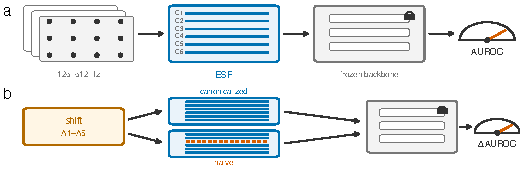
\includegraphics[width=\columnwidth]{fig1_overview.pdf}
\caption{\textbf{Deployment and protocol.} (a)~Recorders that differ in
rate, channel set, gain, mains and export feed one deterministic
six-step contract (ESF) and one frozen model and classifier; nothing
downstream is retrained. (b)~An acquisition operator acts on the raw
microvolt recording; the canonicalized arm applies the full contract,
the naive arm the same contract with the one stage that addresses the
axis switched off; both feed the same frozen model, so their
difference is the recovery attributable to that step.}
\label{fig:overview}
\end{figure}

\section{Background}
\label{sec:background}
BIOT tokenizes heterogeneous biosignals~\cite{yang2023biot}, LaBraM
scales masked-token pretraining to $2{,}500$\,h~\cite{jiang2024labram},
EEGPT adds representation alignment~\cite{wang2024eegpt}; linear
probing of a frozen backbone is the standard
evaluation~\cite{kornblith2019better}. The in-corpus to deployment gap
defines clinical machine
learning~\cite{zech2018variable,finlayson2021clinician,koh2021wilds};
ImageNet-C~\cite{hendrycks2019benchmarking} set the parameterized
perturbation methodology adapted here. BIDS-EEG~\cite{pernet2019bids}
and NWB~\cite{rubel2022nwb} standardize datasets; ESF standardizes the
signal a model sees. Three contemporaneous lines work from the model
side: BRIDGE-EEG~\cite{chowdhury2026bridge} maps recordings to a
device-agnostic $62$-channel time--frequency representation before
pretraining its own encoders; PRISM~\cite{prism2026} pretrains across
acquisition systems; graph montage
harmonization~\cite{gcnharmonization2026} learns a mapping between
electrode layouts. None simulates the recorder as operators, holds a
fixed contract on the other side, ablates it stage by stage, or
measures third-party backbones (Table~S7).

\section{Methods}
\label{sec:methods}

\subsection{Data}
\label{sec:data}
Probes are trained on the TUAB v3.0.1 \emph{train}
split~\cite{lopez2015abnormal,buckwalter2021tuh} ($2{,}717$ recordings,
$2{,}076$ patients; patient-stratified $90/10$ train/validation, seed
$7$) and evaluated once on the official \emph{eval} split ($n{=}276$,
$253$ patients, $150$ normal, $126$ abnormal; patient-ID intersection
with train $0$). No evaluation recording touches training, validation,
calibration or the fixed-scale constants of the naive gain arm.

\subsection{Models, adapters and classifiers}
\label{sec:backbone}
Three frozen public models (backbones) via braindecode~1.5.2: EEGPT
(\texttt{eegpt-pretrained}), LaBraM (\texttt{labram-pretrained}) and
BIOT (\texttt{biot-pretrained-prest-16chs}). Each consumes ESF through
a fixed model-side adapter applied identically to every arm and cell:
EEGPT, $19$ channels at $250$\,Hz in $4$\,s windows, encoder tokens
averaged to $512$-d; LaBraM, $19$ named channels at $200$\,Hz in its
pretrained $15$\,s windows, patch tokens averaged to $200$-d; BIOT, the
$16$ longitudinal bipolar derivations formed from the $19$ referential
channels at $200$\,Hz in $5$\,s windows, $256$-d encoder embedding.
EEGPT's public checkpoint lacks its $19{\to}19$ channel projection; it
is initialised from seed $7$, frozen and released. Each backbone
carries four probes on the pooled per-recording representation (mean,
max, 95th percentile of $\ell_2$-normalised window vectors): three MLP
probes ($3d{\to}256{\to}1$, dropout $0.2$, seeds $7/11/13$, AdamW
$10^{-3}$, class-weighted BCE, $25$ epochs, best validation AUROC) and
one logistic probe; train-statistics standardisation, Platt scaling on
validation. Windows are pooled in up to eight groups; the recording
score is the mean group logit and the across-group variance is kept as
a label-free monitoring statistic.

\subsection{Pretraining provenance}
\label{sec:provenance}
Evaluation recordings must be unseen at every stage, including
pretraining. EEGPT was pretrained on non-TUH data \EEGPTPRETRAIN.
LaBraM's pretraining includes TUAR, TUEP, TUSZ and TUSL but excludes
TUAB and TUEV, recording-disjointly; patient-level overlap with TUAB is
not reported and is a residual, unquantified risk for LaBraM only. For
BIOT we use the checkpoint pretrained on Massachusetts General Hospital
resting EEG alone; the six-dataset checkpoint, which includes TUAB
train, is not used.

\subsection{The contract}
\label{sec:esf}
ESF v1.0: \textbf{(C1)} the $19$ international $10$--$20$
sites~\cite{klem1999tenten} in fixed order; \textbf{(C2)} $250$\,Hz by
anti-aliased polyphase resampling; \textbf{(C3)} physical microvolts
from the EDF header, then channel-wise robust z-score (median, IQR,
persisted); \textbf{(C4)} common average reference over good channels;
\textbf{(C5)} IIR notch at the regional mains and harmonics, and a
$0.5$\,Hz high-pass; \textbf{(C6)} missing channels are \texttt{NaN}
with a quality flag, never imputed. Reference implementation: MIT.

\subsection{Acquisition-shift axes}
\label{sec:shift_model}
Every simulated difference is applied as an operator $A_\theta$ on
the \emph{raw} microvolt recording at its native rate, before any
contract step (Fig.~\ref{fig:overview}b; Table~S6). The
\emph{canonicalized} arm then runs C1--C6; the \emph{naive} arm runs
the same pipeline with the one corrective step disabled, so the arms
differ only in that step and share every downstream weight. One
(difference, severity) setting is a \emph{cell}; a model's
\emph{envelope} is the set of cells in which the canonicalized arm
stays within $0.01$ AUROC of the model's clean baseline. \emph{(A1)}~native rate $f_n \in \{128, 200, 250,
256, 512\}$\,Hz by anti-aliased resampling; naive arm presents native
samples as if $250$\,Hz. \emph{(A2)}~scalar gain $g \in \{0.5, 0.75, 1,
1.5, 2\}$; naive arm normalises with fixed train-set scale constants.
\emph{(A3)}~$60$\,Hz mains and harmonics below native Nyquist, mean
peak $a \in \{0, 5, 15, 30, 60\}\,\mu$V, per-electrode log-normal
amplitude ($\sigma{=}0.3$) and random phase; naive arm has the notch
off. \emph{(A4)}~montage \texttt{full19}, \texttt{legacy16} (T3, T4,
T5, T6, Fz, Cz, Pz absent) or \texttt{bipolar18} re-projected to
referential slots; naive arm averages over all $19$ slots with zeros.
\emph{(A5)}~white noise per channel at SNR $\in \{-5, 0, 5, 10,
20\}$\,dB; no corrective stage exists, so the arms coincide. A sixth,
measurement-only axis low-passes the raw recording at $15$--$100$\,Hz
(\S\ref{sec:bandwidth}).

\subsection{Recoverability framework}
\label{sec:framework}
Let $A_\theta$ map a canonical signal to its native-device
representation and $K_\theta$ be a canonicalization operator targeting
$K_\theta \circ A_\theta = \mathrm{id}$; $f$ is the frozen probe and
$\mathcal{A}(f;\mathcal{D})$ its AUROC. An axis is
\emph{$(f,\varepsilon)$-recoverable} iff some $K_\theta$ keeps
$|\mathcal{A}(f \circ K_\theta \circ A_\theta) - \mathcal{A}(f)| \le
\varepsilon$ for every $\theta$ in the support.
\begin{proposition}[Left-invertibility {$\Rightarrow$} recoverability]\label{prop:inv}
If $A_\theta$ admits a left-inverse within the contract, the axis is
$(f,0)$-recoverable for every $f$.
\end{proposition}
\begin{proposition}[Sub-Nyquist irrecoverability]\label{prop:nyq}
If $A_\theta$ is an ideal anti-alias low-pass at $f_n/2$ followed by
decimation with $f_n < 2 f_{\max}$, \emph{and} $f$ depends on content
in $(f_n/2, f_{\max}]$, no $K_\theta$ recovers $f$'s clean AUROC.
\end{proposition}
\begin{theorem}[AUROC--TV bound, class-conditional]\label{thm:tv}
For any bounded-score $f$, with $P|_{\pm}$ the class-conditional score
distributions,
$|\mathcal{A}(f;\mathcal{D}_0) - \mathcal{A}(f;\mathcal{D}_\theta)|
\le \mathrm{TV}(P_0|_{+}, P_\theta|_{+}) + \mathrm{TV}(P_0|_{-}, P_\theta|_{-})
\le \sum_{\pm}\sqrt{\tfrac{1}{2} D_{\mathrm{KL}}(P_\theta|_{\pm} \| P_0|_{\pm})}$.
\end{theorem}
Proposition~\ref{prop:inv} applies to gain and mains.
Proposition~\ref{prop:nyq} is a statement about the classifier, not the
axis. The marginal score distribution, which a deployed system can
observe without labels, is \emph{not} bounded this way (v1 stated a
marginal form with $C(f)\le 4$; that step was invalid). Proofs and a
composability lemma: Appendix~A.

\begin{table*}[t]
\caption{\textbf{Envelope.} Change in AUROC from each model's clean
baseline on TUAB eval ($n{=}276$), per cell and arm, mean over three
MLP seeds; shading is proportional to the loss, saturating at $-0.5$.
Bold: canonicalized-arm cells more than $0.01$ below baseline, i.e.\
outside the envelope. A5 has no corrective stage, so its naive row is
empty. Paired tests per contrast in Table~S4.}
\label{tab:delta}
\centering\scriptsize\setlength{\tabcolsep}{2.4pt}\renewcommand{\arraystretch}{1.35}
\begin{tabular}{@{}llcccc@{\hspace{5pt}}cccc@{\hspace{5pt}}cccc@{\hspace{5pt}}cc@{\hspace{5pt}}ccccc@{}}
\toprule
 & & \multicolumn{4}{c}{A1 rate (Hz)} & \multicolumn{4}{c}{A2 gain ($\times$)} & \multicolumn{4}{c}{A3 mains ($\mu$V)} & \multicolumn{2}{c}{A4 montage} & \multicolumn{5}{c}{A5 SNR (dB)} \\
 & & 128 & 200 & 256 & 512 & 0.5 & 0.75 & 1.5 & 2 & 5 & 15 & 30 & 60 & leg16 & bip18 & -5 & 0 & 5 & 10 & 20 \\
\midrule
\textcolor{coleegpt}{\textbf{EEGPT}} & naive & \cellcolor{loss!34}$-$0.17 & \cellcolor{loss!4}$-$0.02 & \cellcolor{loss!2}$-$0.01 & \cellcolor{loss!35}$-$0.17 & \cellcolor{loss!16}$-$0.08 & \cellcolor{loss!9}$-$0.04 & \cellcolor{loss!3}$-$0.02 & \cellcolor{loss!4}$-$0.02 & \cellcolor{loss!4}$-$0.02 & \cellcolor{loss!20}$-$0.10 & \cellcolor{loss!43}$-$0.22 & \cellcolor{loss!60}\color{white}$-$0.30 & \cellcolor{loss!1}$-$0.01 & \cellcolor{loss!4}$-$0.02 & \cellcolor{gray!12} & \cellcolor{gray!12} & \cellcolor{gray!12} & \cellcolor{gray!12} & \cellcolor{gray!12} \\
 & canonicalized & \cellcolor{loss!0}0 & \cellcolor{loss!0}0 & \cellcolor{loss!0}0 & \cellcolor{loss!0}0 & \cellcolor{loss!0}0 & \cellcolor{loss!0}0 & \cellcolor{loss!0}0 & \cellcolor{loss!0}0 & \cellcolor{loss!0}0 & \cellcolor{loss!0}0 & \cellcolor{loss!0}0 & \cellcolor{loss!0}0 & \cellcolor{loss!2}\textbf{$-$0.01} & \cellcolor{loss!4}\textbf{$-$0.02} & \cellcolor{loss!33}\textbf{$-$0.16} & \cellcolor{loss!22}\textbf{$-$0.11} & \cellcolor{loss!12}\textbf{$-$0.06} & \cellcolor{loss!8}\textbf{$-$0.04} & \cellcolor{loss!2}\textbf{$-$0.01} \\
\addlinespace[3pt]
\textcolor{collabram}{\textbf{LaBraM}} & naive & \cellcolor{loss!16}$-$0.08 & \cellcolor{loss!10}$-$0.05 & \cellcolor{loss!1}$-$0.01 & \cellcolor{loss!57}\color{white}$-$0.29 & \cellcolor{loss!4}$-$0.02 & \cellcolor{loss!3}$-$0.02 & \cellcolor{loss!2}$-$0.01 & \cellcolor{loss!2}$-$0.01 & \cellcolor{loss!6}$-$0.03 & \cellcolor{loss!19}$-$0.09 & \cellcolor{loss!22}$-$0.11 & \cellcolor{loss!43}$-$0.21 & \cellcolor{loss!9}$-$0.04 & \cellcolor{loss!4}$-$0.02 & \cellcolor{gray!12} & \cellcolor{gray!12} & \cellcolor{gray!12} & \cellcolor{gray!12} & \cellcolor{gray!12} \\
 & canonicalized & \cellcolor{loss!16}\textbf{$-$0.08} & \cellcolor{loss!0}0 & \cellcolor{loss!0}0 & \cellcolor{loss!0}0 & \cellcolor{loss!0}0 & \cellcolor{loss!0}0 & \cellcolor{loss!0}0 & \cellcolor{loss!0}0 & \cellcolor{loss!0}0 & \cellcolor{loss!0}0 & \cellcolor{loss!0}0 & \cellcolor{loss!0}0 & \cellcolor{loss!9}\textbf{$-$0.04} & \cellcolor{loss!4}\textbf{$-$0.02} & \cellcolor{loss!41}\textbf{$-$0.20} & \cellcolor{loss!30}\textbf{$-$0.15} & \cellcolor{loss!24}\textbf{$-$0.12} & \cellcolor{loss!17}\textbf{$-$0.09} & \cellcolor{loss!10}\textbf{$-$0.05} \\
\addlinespace[3pt]
\textcolor{colbiot}{\textbf{BIOT}} & naive & \cellcolor{loss!65}\color{white}$-$0.32 & \cellcolor{loss!11}$-$0.05 & \cellcolor{loss!0}0 & \cellcolor{loss!99}\color{white}$-$0.49 & \cellcolor{loss!12}$-$0.06 & \cellcolor{loss!11}$-$0.05 & \cellcolor{loss!5}$-$0.02 & \cellcolor{loss!8}$-$0.04 & \cellcolor{loss!47}$-$0.24 & \cellcolor{loss!53}$-$0.27 & \cellcolor{loss!51}$-$0.25 & \cellcolor{loss!54}$-$0.27 & \cellcolor{loss!5}$-$0.03 & \cellcolor{loss!4}$-$0.02 & \cellcolor{gray!12} & \cellcolor{gray!12} & \cellcolor{gray!12} & \cellcolor{gray!12} & \cellcolor{gray!12} \\
 & canonicalized & \cellcolor{loss!46}\textbf{$-$0.23} & \cellcolor{loss!1}0 & \cellcolor{loss!0}0 & \cellcolor{loss!0}0 & \cellcolor{loss!0}0 & \cellcolor{loss!0}0 & \cellcolor{loss!0}0 & \cellcolor{loss!0}0 & \cellcolor{loss!0}0 & \cellcolor{loss!0}0 & \cellcolor{loss!0}0 & \cellcolor{loss!0}0 & \cellcolor{loss!6}\textbf{$-$0.03} & \cellcolor{loss!4}\textbf{$-$0.02} & \cellcolor{loss!44}\textbf{$-$0.22} & \cellcolor{loss!23}\textbf{$-$0.11} & \cellcolor{loss!18}\textbf{$-$0.09} & \cellcolor{loss!11}\textbf{$-$0.06} & \cellcolor{loss!10}\textbf{$-$0.05} \\
\bottomrule
\end{tabular}

\end{table*}

\subsection{Statistics}
\label{sec:stats}
Canonicalized-vs-naive contrasts use DeLong's test on matched
recordings~\cite{delong1988comparing}; intervals are paired
class-stratified bootstraps ($1{,}000$ resamples); Benjamini--Hochberg
at $q{=}0.05$ over the non-identity cells of each
backbone~\cite{benjamini1995controlling}. Tables report the mean over
the three MLP seeds; tests use the seed-7 probe.

\section{Results}
\label{sec:results}

\subsection{Baselines and per-axis results}
\label{sec:axes}
On clean recordings the three models are equally good: AUROC $0.900$
(EEGPT), $0.894$ (LaBraM) and $0.898$ (BIOT), each within $0.01$ across
classifier seeds. Table~\ref{tab:delta} gives every cell;
Fig.~\ref{fig:cells}a adds the seed spread; Tables~S1--S4 add balanced
accuracy, expected calibration error (ECE) and paired tests.

\textit{Sampling rate (A1).} Resampling to $250$\,Hz undoes every rate
for EEGPT, including $128$\,Hz, where the naive arm had lost $0.17$.
For BIOT and LaBraM it undoes $200$, $256$ and $512$\,Hz (the naive
$512$\,Hz arm of BIOT is below chance) but not $128$\,Hz: BIOT falls
from $0.90$ to $0.67$ and LaBraM from $0.89$ to $0.82$ whether or not
the signal is resampled, and both push normal recordings toward
abnormal. What is lost at $128$\,Hz is signal content above $64$\,Hz,
and \S\ref{sec:bandwidth} shows which models use it.

\textit{Gain (A2).} Per-recording robust scaling undoes any gain for
every model. Without it, EEGPT and BIOT lose up to $0.08$ at half
gain and are already below baseline at unit gain, because fixed
scaling constants are themselves a mis-normalization; LaBraM's naive
arm is largely tolerant.

\textit{Mains interference (A3).} The notch undoes mains at every
amplitude for every model. Without it, EEGPT loses $0.30$ and BIOT
$0.27$ at $60\,\mu$V, and from $15\,\mu$V both call almost every
recording abnormal; LaBraM loses $0.21$ and, unlike the other two,
drifts toward calling recordings normal (\S\ref{sec:failure}).

\textit{Electrode montage (A4).} Neither averaging over the present
electrodes nor averaging over all $19$ recovers the missing ones. The
loss is small for EEGPT ($0.01$--$0.02$) and larger for LaBraM
($0.04$ on \texttt{legacy16}, with balanced accuracy near chance); it
is in the acquisition, not the reference.

\textit{Broadband noise (A5).} There is no corrective step, so the
arms coincide and AUROC falls with signal-to-noise ratio for every
model, most steeply for BIOT and LaBraM.

\begin{figure*}[t]
\centering
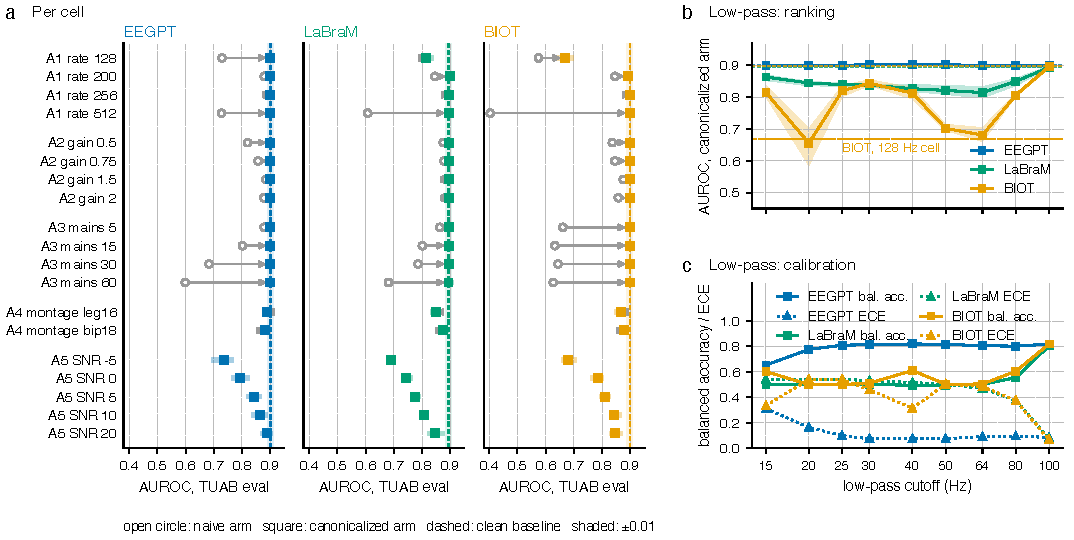
\includegraphics[width=\textwidth]{fig2_cells_bandwidth.pdf}
\caption{\textbf{Every cell, and why the models disagree.}
(a)~AUROC of the naive arm (open circle) and the canonicalized arm
(filled square) per model; the arrow is the recovery the stage
delivers, the band the min--max over three probe seeds, the shaded
strip the $\pm 0.01$ envelope around the clean baseline. (b)~AUROC of
the canonicalized arm after a low-pass applied to the raw recording:
EEGPT's ranking is unchanged down to $15$\,Hz; BIOT's and LaBraM's
$64$\,Hz cells reproduce their $128$\,Hz cells with no resampling.
(c)~Balanced accuracy and ECE over the same cutoffs.}
\label{fig:cells}
\end{figure*}

\subsection{Bandwidth is a property of the model}
\label{sec:bandwidth}
To find out which models use the content that low-rate acquisition
removes, we low-pass the raw recording at cutoffs from $15$ to
$100$\,Hz before the contract (Fig.~\ref{fig:cells}b,c). EEGPT's
ranking does not change at any cutoff, so nothing above $15$\,Hz
enters its decision; its calibration does change below $30$\,Hz
(balanced accuracy $0.81 \to 0.65$). BIOT and LaBraM lose accuracy as
soon as the cutoff drops below $100$\,Hz, and their $64$\,Hz cells
reproduce their $128$\,Hz cells exactly ($0.68$ and $0.82$). Both were
pretrained on $200$\,Hz input and tokenize the $64$--$100$\,Hz band;
EEGPT works on time-domain patches and does not. For deployment the
envelope therefore has two edges, one for ranking and a tighter one
for calibrated decisions.

\subsection{How individual recordings fail}
\label{sec:failure}
Aggregate AUROC hides what happens to a given recording, so we follow
each one across the $12$ non-identity cells of the rate, gain and
mains axes and sort it into one of seven categories
(Fig.~\ref{fig:recordings}c; Table~S5). The category that matters is
\emph{catastrophic shift}: a recording the model gets right on clean
data and then, on at least one cell, gets wrong with probability
$0.80$ or more. Without the contract, this happens to every correctly
classified normal recording for EEGPT ($110/110$) and BIOT
($124/124$), almost always toward a confident abnormal report; for
LaBraM it happens to normals at $512$\,Hz ($104/119$) and, in the
opposite direction, to abnormals under mains interference ($90/103$
at $60\,\mu$V). Which way a model fails is therefore a property of the
model and the difference together; for a screening tool the first
direction costs review time~\cite{ghassemi2021false}, the second costs
missed disease. With the contract, no confident flip remains for
EEGPT, and none for BIOT or LaBraM outside the $128$\,Hz cell, where
$100$ of $124$ and $79$ of $119$ correctly classified normals still
flip. ``Flips on some cell'' is a maximum over $12$ cells and
describes this sweep, not a population rate.

\begin{figure*}[t]
\centering
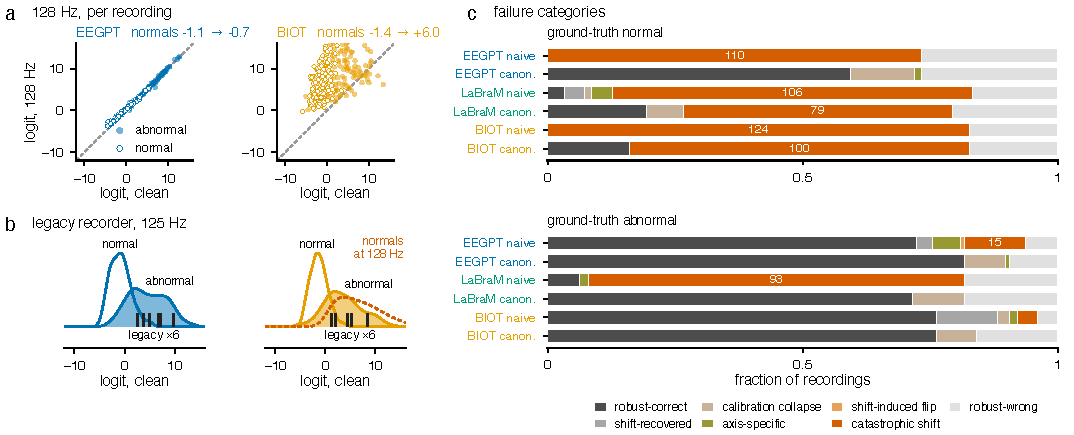
\includegraphics[width=\textwidth]{fig3_recordings.pdf}
\caption{\textbf{What the envelope means for a recording, a population
and a recorder.} (a)~Per-recording logit after $128$\,Hz acquisition
and the full contract against the clean logit (seed-7 probes): EEGPT
stays on the identity, BIOT lifts every normal recording by about
$7$ logits. (b)~Clean eval logit distributions with the six legacy
Natus recordings ($125$\,Hz) as ticks; for BIOT the dashed curve is
where its eval normals land at this rate. (c)~Failure-category
composition over the $12$ non-identity cells of A1--A3, by model, arm and ground truth (counts in Table~S5).}
\label{fig:recordings}
\end{figure*}

\subsection{Controls, monitor, bound}
\label{sec:controls}
\textit{Could the classifiers have learned something other than the
label?} Classifiers trained on permuted labels (training and
validation both permuted, ten repeats) score at chance for EEGPT
($0.46 \pm 0.08$) and LaBraM ($0.48 \pm 0.10$) and slightly above it
for BIOT ($0.58 \pm 0.04$). The BIOT residual is not leakage: with no
labels at all, the distance of an evaluation recording from its ten
nearest training recordings already separates the classes at $0.74$
for BIOT ($0.70$ LaBraM, $0.51$ EEGPT), and untrained random
classifiers score at chance. Abnormal recordings are simply atypical
in BIOT's feature space. \textit{Could a deployed system detect the
failures without labels?} Neither the spread of a recording's window
scores nor its distance from a probability of $0.5$ ranks the
catastrophic recordings above the rest (median AUROC $0.54$ over $11$
naive cells); the failures look, to the model, like ordinary
confident decisions. \textit{Bound.} \PINSKERNUMBERS

\subsection{A real legacy recorder}
\label{sec:legacy}
Six de-identified routine recordings from a Natus recorder in clinical
use ($125$\,Hz, $24$--$27$ channels, $50$\,Hz mains, proprietary
\texttt{.e} export; no reads available) were parsed, passed through
the contract and scored locally. All three models call all six
abnormal. The recorder's $125$\,Hz sits inside EEGPT's envelope and
outside LaBraM's and BIOT's (Fig.~\ref{fig:recordings}b), so only
EEGPT's verdict could be tested against reads; whether the six are
abnormal or merely shifted, we do not guess.

\section{Discussion}
\label{sec:discussion}
\textbf{What the contract closes depends on the model.} Gain and
mains are undone for every model, as the theory predicts before any
data. A low sampling rate is undone for EEGPT and not for the other
two, and the low-pass sweep locates the reason in the $64$--$100$\,Hz
band. A contract measured on one model says nothing about another.
Missing electrodes and broadband noise are undone for none; the
practical response is to flag such recordings at intake by the size
of the model's output, since every model fails with high confidence
and a rule based on borderline probabilities would miss exactly these
failures.

\textbf{Changing the contract.} Because EEGPT uses nothing above
$15$\,Hz, ESF v1.1 will add an explicit $0.5$--$50$\,Hz band-limit,
as BRIDGE-EEG's preprocessing does~\cite{chowdhury2026bridge}; for a
model of that bandwidth every native rate from $100$\,Hz upward is
then on-contract by construction. For BIOT or LaBraM the same step
would move the edge, not remove it: a step must be measured per model,
not assumed.

\textbf{Scope.} One task on one public corpus, three frozen models,
small classifiers, simulated rather than sampled recorders, and six
unlabelled clinical recordings. LaBraM's pretraining includes other
TUH subcorpora (\S\ref{sec:provenance}). No clinical claim is made; a
labelled multi-recorder study is the next step (Appendix~E).

\section{Conclusion}
\label{sec:conclusion}
A preprocessing contract can be measured rather than assumed. Five
simulated recorder differences, three frozen models, and each
corrective step switched on and off give, per model, the differences
the contract undoes, the step responsible and the calibration cost.
Uncorrected, the models fail confidently and in model-specific
directions; corrected, they fail only where the sweep says the
contract cannot reach.

\section*{Reproducibility}
\label{sec:repro}
Code, operators, adapters, all probes, feature caches, per-cell
predictions for every (backbone, probe, cell), tables and proofs:
\url{https://github.com/h5371h/esf-recoverability} (MIT; tag
\texttt{v2.0.0-preprint-v2}, archived as doi:10.5281/zenodo.22771925; the
withdrawn v1
snapshot remains at \texttt{v1.0.0-spmb2026-submission}). TUAB is
obtained under the NEDC agreement~\cite{lopez2015abnormal}; the legacy
recordings are clinical data, processed locally and not released.
Checkpoint revisions, library versions and seeds: Appendix~E. Every
number regenerates from the released caches without a GPU.
\textit{Cost.} On a $30$-core CPU the full contract takes $0.64$\,s per
$25$-min recording (notch $0.28$, EDF read $0.23$, robust z $0.17$,
high-pass $0.16$, CAR $0.02$, resample $<0.01$\,s); the backbones take
$12$ (EEGPT), $1.6$ (LaBraM) and $0.5$\,s (BIOT), or $113/10/3$\,s
single-threaded. The contract is never the bottleneck.

\section*{Version note (v2)}
\label{sec:version}
v2 corrects v1 in six respects, all found by the author after
submission: v1 applied operators \emph{after} canonicalization (its
rate axis was a time-warp, its gain arm never composed forward and
inverse, its mains amplitudes were in robust-SD units); its probe was
trained on a split that overlapped eval; Theorem~\ref{thm:tv} was
stated marginally; $C_{\max}$ was fitted, not validated; the
conflict-of-interest statement was incomplete; the channel-projection
adapter was unseeded. \emph{Withdrawn:} the v1 losses at $128$ and
$512$\,Hz for EEGPT, the montage calibration recovery, the empirical
support for Proposition~\ref{prop:nyq}. \emph{Added:} LaBraM, BIOT,
seeds, a linear probe, bandwidth, envelope, controls, the legacy
recorder. Details: Appendix~E.

\section*{Acknowledgements}
No external research funding. v1 compute: Microsoft for Startups
Founders Hub; v2 compute: Lambda Cloud, paid by the author. The author
thanks NEDC for TUAB and the EEGPT, LaBraM and BIOT authors for open
weights. \textbf{Conflict of interest.} The author is the founder of
Aposematium Private Limited, which develops the ENCEPHLIAN clinical-EEG
software; the format described here shares that product's name and the
author has a commercial interest in its adoption. The reference
implementation is MIT-licensed.

\bibliographystyle{IEEEtranN}
\bibliography{SPMB2026_Dammu_final_v4}
\end{document}
